\documentclass[12pt]{article}
\usepackage[margin=1.2in]{geometry}
\usepackage{amsmath}
\usepackage{graphicx}
\usepackage{caption}
\usepackage{subcaption}
\begin{document}
\title{COL334 - Assignment 1\\ Internet Architecture}
\author{Akshay Kumar Gupta\\\texttt{2013CS50275} \and  Barun Patra\\\texttt{2013CS10773} \and Haroun Habeeb\\\texttt{2013CS10225}}
\date{}
\maketitle
\noindent {\bfseries Q4a.} List of applications generating background traffic:
\begin{itemize}
\item Adobe Creative Cloud
\item Pushbullet
\item WifiAgent
\item TextMate
\item Spotify
\end{itemize}
~\\
{\bfseries Q4b.} Analysis of internal IITD webpage download after clearing local DNS cache:
\begin{itemize}
\item Servers for which a DNS query was launched: 10.10.1.2 or 10.7.174.111
\item Number of HTTP requests generated: 60 
\item Number of TCP connections opened: 7
\item Time taken for downloading webpage: $\sim$ 1 second
\item No. of TCP losses / retransmits: 0
\end{itemize}
\begin{figure}[h!]
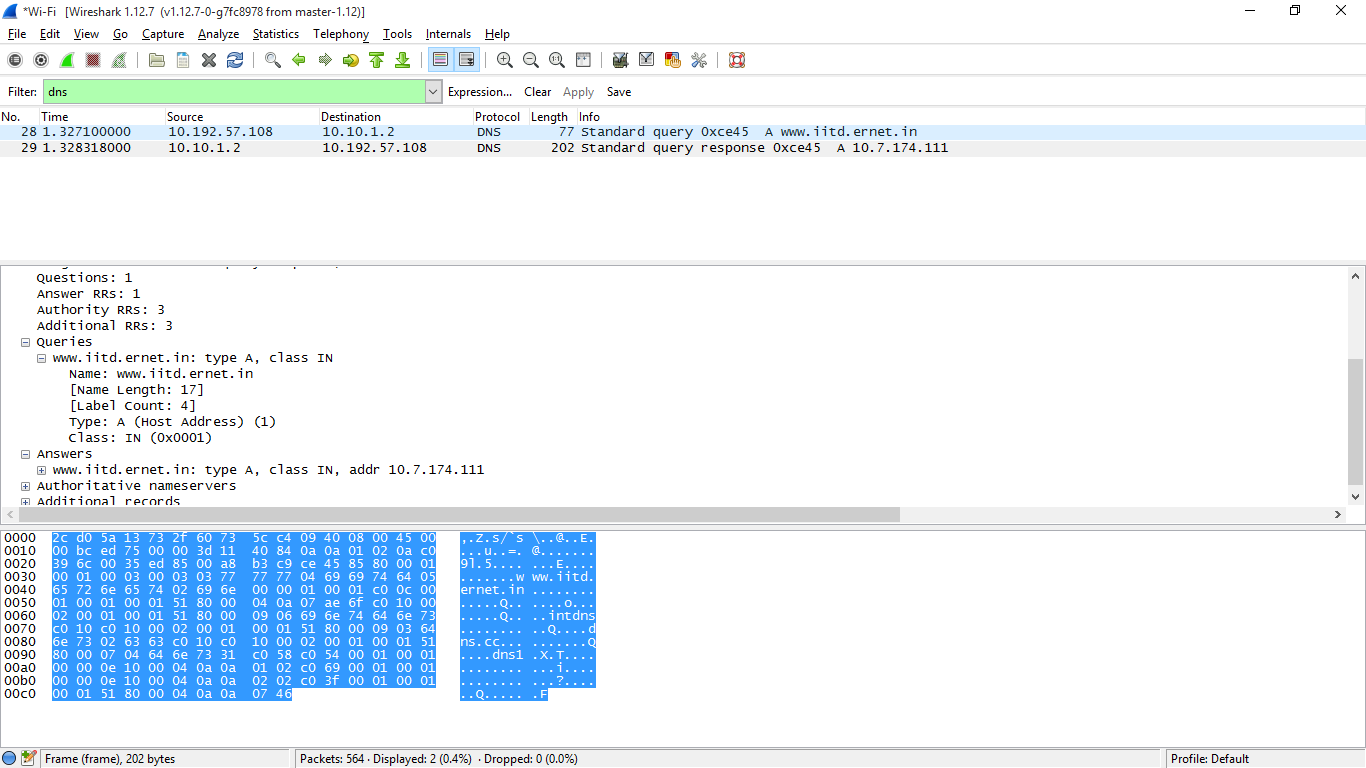
\includegraphics[scale=0.38]{../Screenshots/dns-reply2.png}
\caption{DNS Query}
\end{figure}
~\\
\begin{figure}[h!]
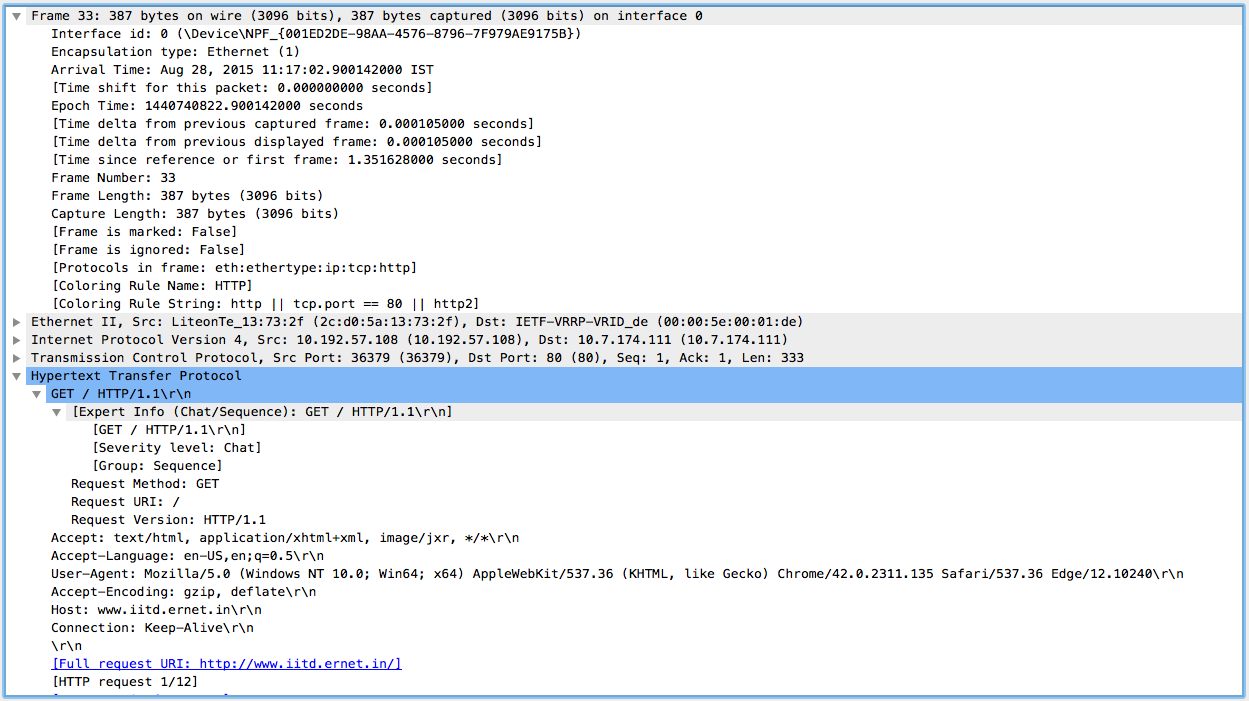
\includegraphics[scale=0.38]{../Screenshots/http-get-request.png}
\caption{HTTP Get Request}
\end{figure}
\begin{figure}[h!]
\centerline {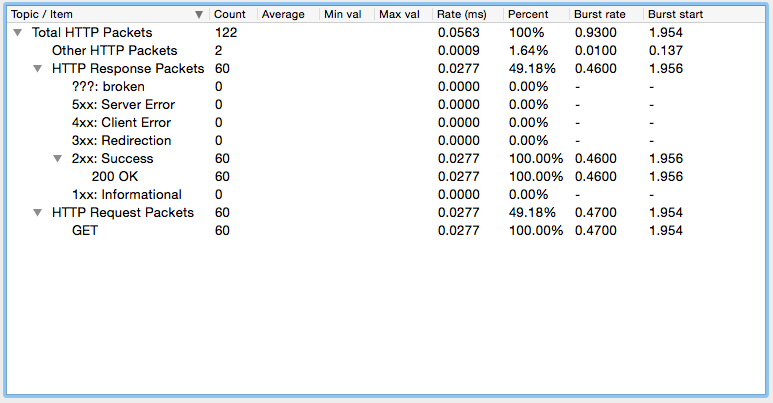
\includegraphics[scale=0.4]{../Screenshots/num-http-requests.png}}
\caption{Number of HTTP requests}
\end{figure}
~\\
\begin{figure}[h]
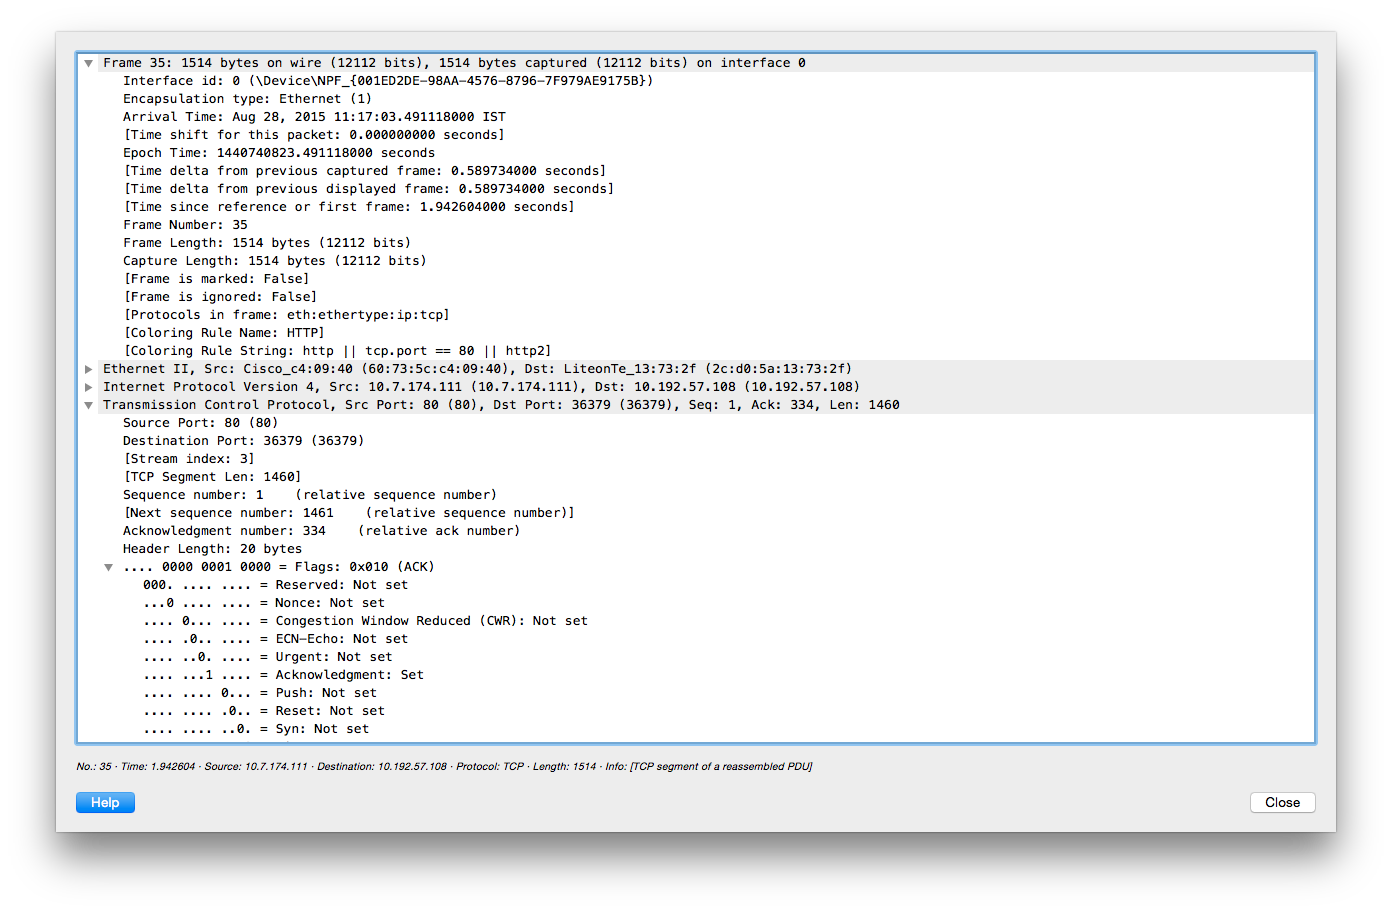
\includegraphics[scale=0.38]{../Screenshots/tcp-header.png}
\caption{TCP Header}
\end{figure}
\begin{figure}[h!]
\centering
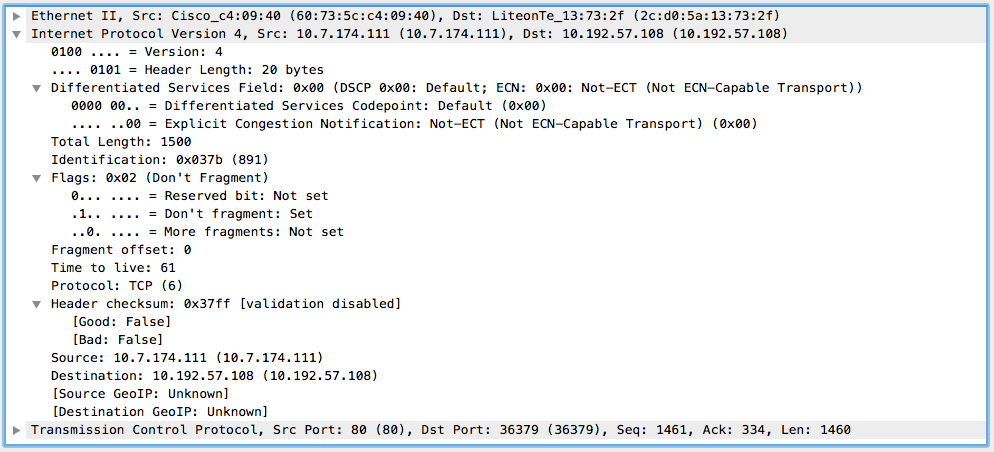
\includegraphics[scale=0.5]{../Screenshots/ip-header.png}
\caption{IP Header}
\end{figure}
\begin{figure}[h!]
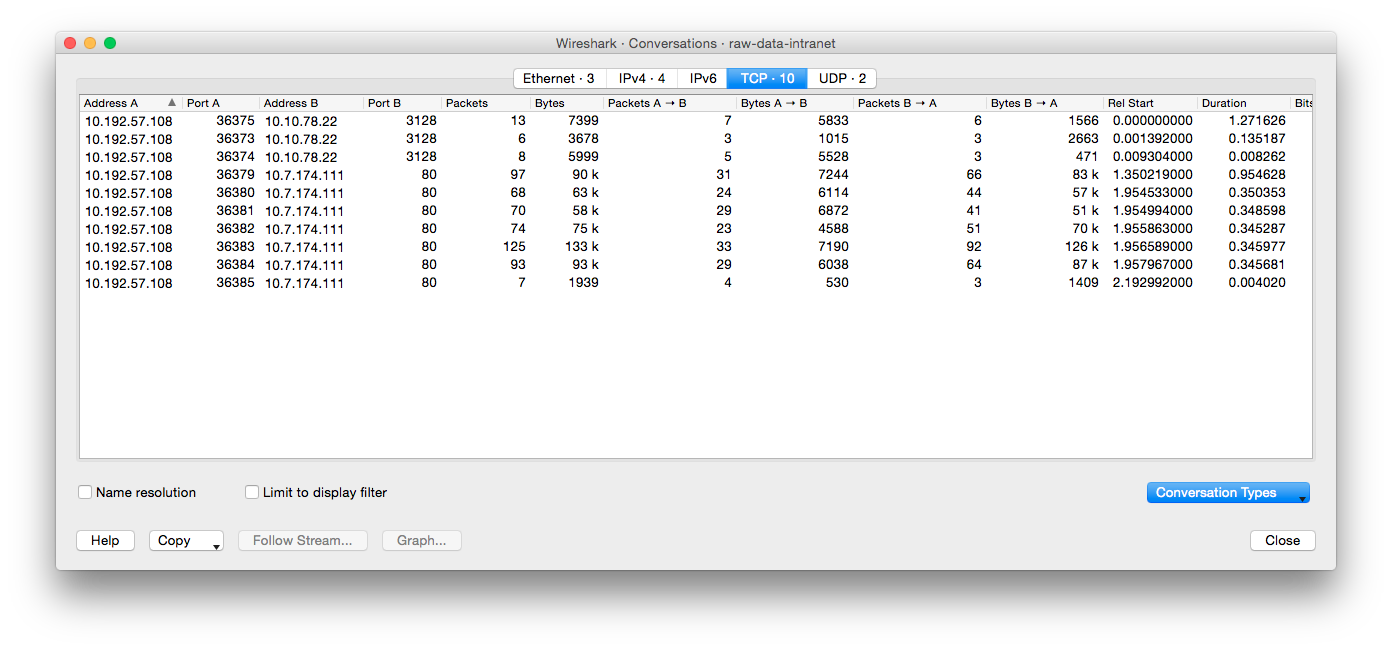
\includegraphics[scale=0.39]{../Screenshots/tcp-connections.png}
\caption{TCP Connections}
\end{figure}
\end{document}